\documentclass{article}%
\usepackage{amsmath}
\usepackage{amsfonts}
\usepackage{amssymb}
\usepackage{listings}
\usepackage{graphicx}
\usepackage{tikz}
\usepackage{hyperref}%
\usepackage[a4paper,includeheadfoot,margin=0.5in]{geometry}
\setcounter{MaxMatrixCols}{30}
%TCIDATA{OutputFilter=late$x2$.dll}
%TCIDATA{Version=5.00.0.2552}
%TCIDATA{CSTFile=40 LaTeX article.cst}
%TCIDATA{Created=Thursday, August 21, 2008 14:03:59}
%TCIDATA{LastRevised=Wednesday, October 01, 2014 12:46:33}
%TCIDATA{<META NAME="GraphicsSave" CONTENT="32">}
%TCIDATA{<META NAME="SaveForMode" CONTENT="1">}
%TCIDATA{<META NAME="DocumentShell" CONTENT="Standard LaTeX\Blank - Standard LaTeX Article">}
%TCIDATA{Language=American English}
\newtheorem{theorem}{Theorem}
\newtheorem{acknowledgement}[theorem]{Acknowledgement}
\newtheorem{algorithm}[theorem]{Algorithm}
\newtheorem{axiom}[theorem]{Axiom}
\newtheorem{case}[theorem]{Case}
\newtheorem{claim}[theorem]{Claim}
\newtheorem{conclusion}[theorem]{Conclusion}
\newtheorem{condition}[theorem]{Condition}
\newtheorem{conjecture}[theorem]{Conjecture}
\newtheorem{corollary}[theorem]{Corollary}
\newtheorem{criterion}[theorem]{Criterion}
\newtheorem{definition}[theorem]{Definition}
\newtheorem{example}[theorem]{Example}
\newtheorem{exercise}[theorem]{Exercise}
\newtheorem{lemma}[theorem]{Lemma}
\newtheorem{notation}[theorem]{Notation}
\newtheorem{problem}[theorem]{Problem}
\newtheorem{proposition}[theorem]{Proposition}
\newtheorem{remark}[theorem]{Remark}
\newtheorem{solution}[theorem]{Solution}
\newtheorem{summary}[theorem]{Summary}
\newenvironment{proof}[1][Proof]{\noindent\textbf{#1.} }{\ \rule{0.5em}{0.5em}}

\usepackage{fancyhdr}
\setlength\headheight{26pt}
\pagestyle{fancy}
\lhead{{\footnotesize Assignment 13}}
\rhead{{\footnotesize Christopher Chapline}}
\begin{document}

\section*{Problem 1}
$S \rightarrow bA$ \\
\\
$S \rightarrow A$ \\
\\
$A \rightarrow aA$ \\
\\
$A \rightarrow \epsilon$

\section*{Problem 2}
\begin{tikzpicture}[scale=0.2]
    \tikzstyle{every node}+=[inner sep=0pt]
    \draw [black] (17.2,-25.9) circle (3);
    \draw (17.2,-25.9) node {$q_0$};
    \draw [black] (56.2,-25.9) circle (3);
    \draw (56.2,-25.9) node {$q_2$};
    \draw [black] (56.2,-25.9) circle (2.4);
    \draw [black] (36,-25.9) circle (3);
    \draw (36,-25.9) node {$q_1$};
    \draw [black] (36,-25.9) circle (2.4);
    \draw [black] (19.756,-24.332) arc (119.06776:60.93224:34.875);
    \fill [black] (53.64,-24.33) -- (53.19,-23.51) -- (52.7,-24.38);
    \draw (36.7,-19.44) node [above] {$a$};
    \draw [black] (58.88,-24.577) arc (144:-144:2.25);
    \draw (63.45,-25.9) node [right] {$a$};
    \fill [black] (58.88,-27.22) -- (59.23,-28.1) -- (59.82,-27.29);
    \draw [black] (20.2,-25.9) -- (33,-25.9);
    \fill [black] (33,-25.9) -- (32.2,-25.4) -- (32.2,-26.4);
    \draw (26.6,-25.4) node [above] {$b$};
    \draw [black] (39,-25.9) -- (53.2,-25.9);
    \fill [black] (53.2,-25.9) -- (52.4,-25.4) -- (52.4,-26.4);
    \draw (46.1,-25.4) node [above] {$a$};
    \draw [black] (11.2,-25.9) -- (14.2,-25.9);
    \draw (10.7,-25.9) node [left] {$start$};
    \fill [black] (14.2,-25.9) -- (13.4,-25.4) -- (13.4,-26.4);
\end{tikzpicture}

\section*{Problem 3}
$S \rightarrow abcS$ \\
\\
$S \rightarrow \epsilon$

\section*{Problem 4}
\begin{tikzpicture}[scale=0.2]
    \tikzstyle{every node}+=[inner sep=0pt]
    \draw [black] (22.7,-31.8) circle (3);
    \draw (22.7,-31.8) node {$q_0$};
    \draw [black] (22.7,-31.8) circle (2.4);
    \draw [black] (36.4,-31.8) circle (3);
    \draw (36.4,-31.8) node {$q_1$};
    \draw [black] (51,-31.8) circle (3);
    \draw (51,-31.8) node {$q_2$};
    \draw [black] (25.7,-31.8) -- (33.4,-31.8);
    \fill [black] (33.4,-31.8) -- (32.6,-31.3) -- (32.6,-32.3);
    \draw (29.55,-32.3) node [below] {$a$};
    \draw [black] (39.4,-31.8) -- (48,-31.8);
    \fill [black] (48,-31.8) -- (47.2,-31.3) -- (47.2,-32.3);
    \draw (43.7,-32.3) node [below] {$b$};
    \draw [black] (25.165,-30.095) arc (120.89526:59.10474:22.756);
    \fill [black] (25.17,-30.09) -- (26.11,-30.11) -- (25.6,-29.25);
    \draw (36.85,-26.37) node [above] {$c$};
    \draw [black] (16.5,-31.8) -- (19.7,-31.8);
    \draw (16,-31.8) node [left] {$start$};
    \fill [black] (19.7,-31.8) -- (18.9,-31.3) -- (18.9,-32.3);
\end{tikzpicture}

\section*{Problem 5}
$S \rightarrow aA$ \\
\\
$A \rightarrow aaA$ \\
\\
$A \rightarrow \epsilon$

\section*{Problem 6}
\begin{tikzpicture}[scale=0.2]
    \tikzstyle{every node}+=[inner sep=0pt]
    \draw [black] (29.6,-25.3) circle (3);
    \draw (29.6,-25.3) node {$q_0$};
    \draw [black] (42.4,-25.3) circle (3);
    \draw (42.4,-25.3) node {$q_1$};
    \draw [black] (42.4,-25.3) circle (2.4);
    \draw [black] (57.1,-25.3) circle (3);
    \draw (57.1,-25.3) node {$q_2$};
    \draw [black] (32.6,-25.3) -- (39.4,-25.3);
    \fill [black] (39.4,-25.3) -- (38.6,-24.8) -- (38.6,-25.8);
    \draw (36,-25.8) node [below] {$a$};
    \draw [black] (44.054,-22.818) arc (135.54219:44.45781:7.98);
    \fill [black] (55.45,-22.82) -- (55.24,-21.9) -- (54.53,-22.6);
    \draw (49.75,-19.93) node [above] {$a$};
    \draw [black] (55.548,-27.846) arc (-42.32444:-137.67556:7.842);
    \fill [black] (43.95,-27.85) -- (44.12,-28.77) -- (44.86,-28.1);
    \draw (49.75,-30.91) node [below] {$a$};
    \draw [black] (22.4,-25.3) -- (26.6,-25.3);
    \draw (21.9,-25.3) node [left] {$start$};
    \fill [black] (26.6,-25.3) -- (25.8,-24.8) -- (25.8,-25.8);
\end{tikzpicture}


\end{document}
